%
% File acl2017.tex
%
%% Based on the style files for ACL-2015, with some improvements
%%  taken from the NAACL-2016 style
%% Based on the style files for ACL-2014, which were, in turn,
%% based on ACL-2013, ACL-2012, ACL-2011, ACL-2010, ACL-IJCNLP-2009,
%% EACL-2009, IJCNLP-2008...
%% Based on the style files for EACL 2006 by 
%%e.agirre@ehu.es or Sergi.Balari@uab.es
%% and that of ACL 08 by Joakim Nivre and Noah Smith

\documentclass[11pt,a4paper]{article}
\usepackage[hyperref]{acl2017}
\usepackage{times}
\usepackage{latexsym}
\usepackage{graphicx}
\usepackage{float}

\usepackage{url}

\aclfinalcopy % Uncomment this line for the final submission
%\def\aclpaperid{***} %  Enter the acl Paper ID here

%\setlength\titlebox{5cm}
% You can expand the titlebox if you need extra space
% to show all the authors. Please do not make the titlebox
% smaller than 5cm (the original size); we will check this
% in the camera-ready version and ask you to change it back.

\newcommand\BibTeX{B{\sc ib}\TeX}

\title{Verb Duration Bench Mark}

\author{Xiang Yuanxin}


\date{01}

\begin{document}
\maketitle

\begin{abstract}
This task aims to propose a bench mark of the verb duration project. Firstly, I extract frames and frame+verbs and their corresponding durations from the training data to form a corpus. Secondly, I am trying to evaluate the degree of relevance between frames and durations. The result shows that there are some relationships between frames and durations, but these relationships are not strong. However, this conclusion is limited by the Insufficient data. Thirdly, I compute the confusion matrix and analyze the result. 
\end{abstract}


\section{Preparing data}

The FrameNet has annotated some continuous texts and there are 10147 sentences in total. However, of these sentences, there are only 553 sentences explicitly contain duration information and these sentences form our dataset. I randomly select 20 percent of the total sentences to be the testing dataset. So the training dataset contains 443 sentences and the testing dataset contains 110 sentences.
I use tool Sutime to discover sentences which explicitly contain duration information. Sutime is a library for recognizing and normalizing time expressions. And the normalized time expressions are: PT*S, PT*M, PT*H, P*D, P*W, P*M, P*Y and they are corresponding to Seconds, Minutes, Hours, Days, Weeks, Months, Years. In most situation, Sutime can correctly recognize and normalize time expressions, but sometimes it may fail to normalize time expressions. Figure1 gives some examples.



\begin{figure}[H] 
\begin{center} 
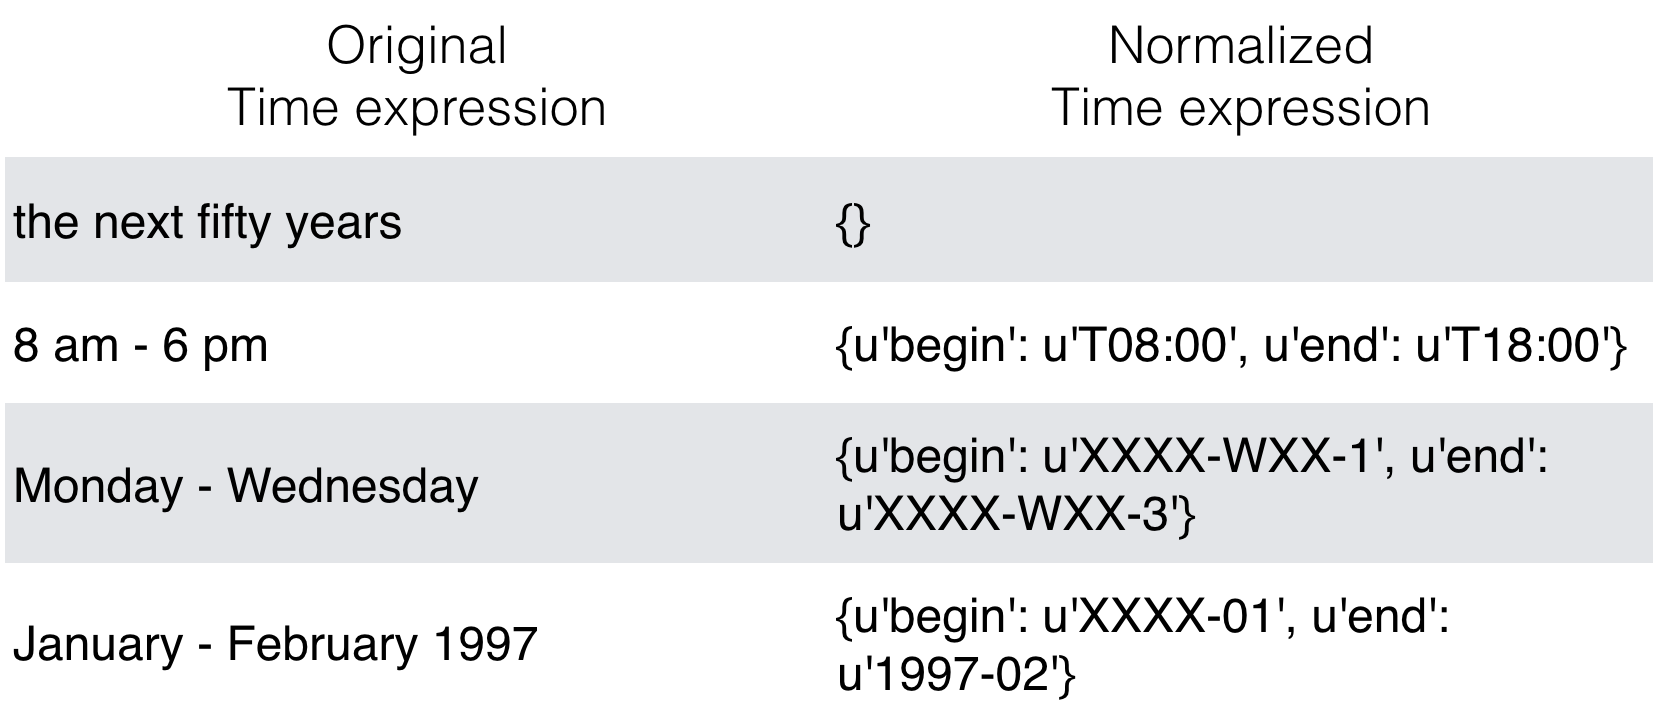
\includegraphics[width=\columnwidth]{figs/fig1.png}
\caption{Some examples of failing to normalize time expression.}
\label{first_fig}
\end{center}
\vskip -0.3in
\end{figure}


Because our dataset is already very small, I can not just throw these failing ones away. So I use some simple but useful rules to correct these failing ones. The priority is from top to bottom.

\textbf{1)} If original time expression mentions "am" or "pm", I consider the duration most likely to be "Hours".

\textbf{2)} If original time expression mentions "Monday", "Tuesday" ... "Sunday", I consider the duration most likely to be "Days"

\textbf{3)} If original time expression mentions "January", "February" ... "December", I consider the duration most likely to be "Months"

\textbf{4)} If original time expression mentions "year", I consider the duration most likely to be "Years"

After this step, the data looks like:

\begin{figure}[H] 
\begin{center} 
\centerline{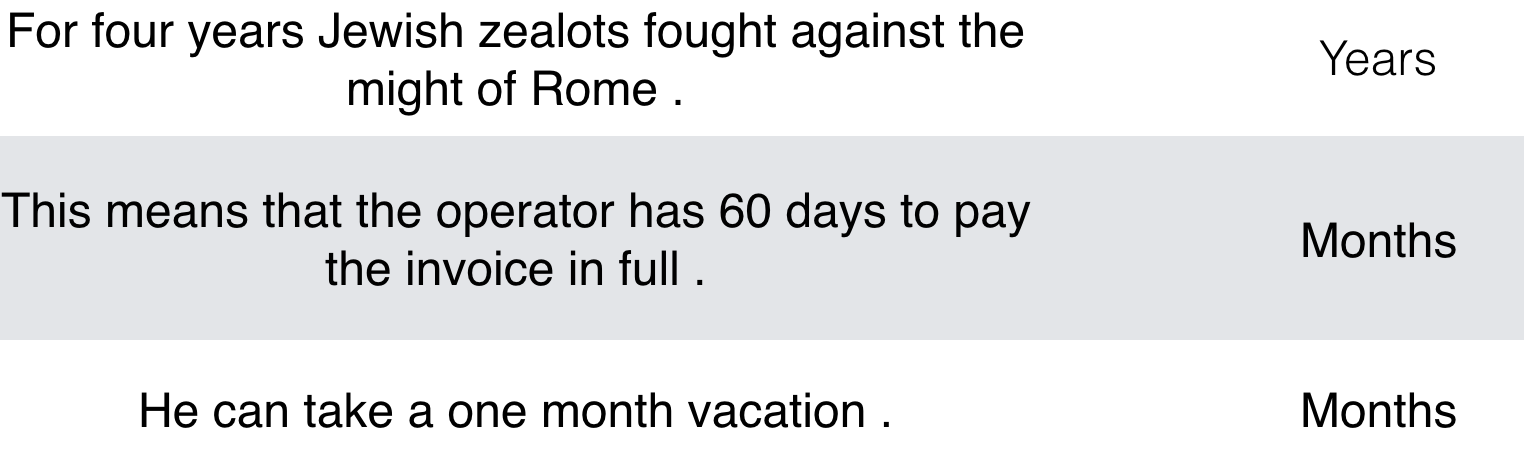
\includegraphics[width=\columnwidth]{figs/fig2.png}}
\caption{Sentences that have been correctly annotated duration.}
\label{second_fig}
\end{center}
\vskip -0.3in
\end{figure}


\section{Extract frame and frame+verb duration}

After preparing data, I use FrameNet to discover that the frames' and frame-verbs' durations. There are some rules to choose the most proper duration.

\textbf{1)} If a frame corresponds to more than one durations, I select the duration that appears most frequently.

\textbf{2)} If more than one duration appears equal times, I select the smallest duration.

The frame+verb and frame duration data looks like:

\begin{figure}[H] 
\begin{center} 
\centerline{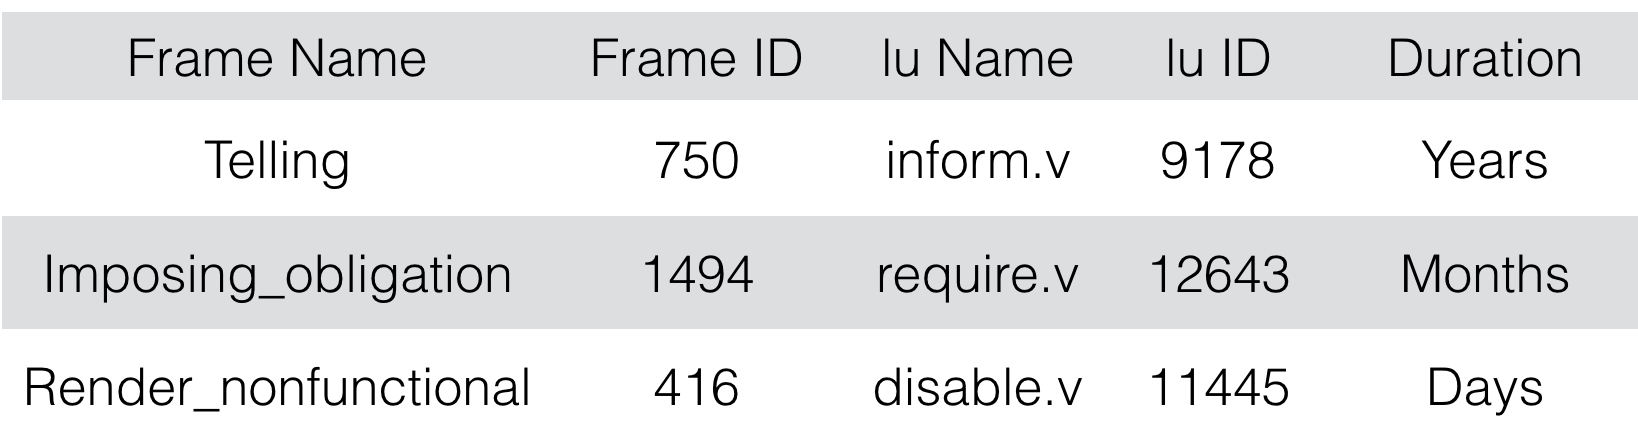
\includegraphics[width=\columnwidth]{figs/fig3.png}}
\caption{Frame+verb duration.}
\label{third_fig}
\end{center}
\vskip -0.3in
\end{figure}


\begin{figure}[H] 
\begin{center} 
\centerline{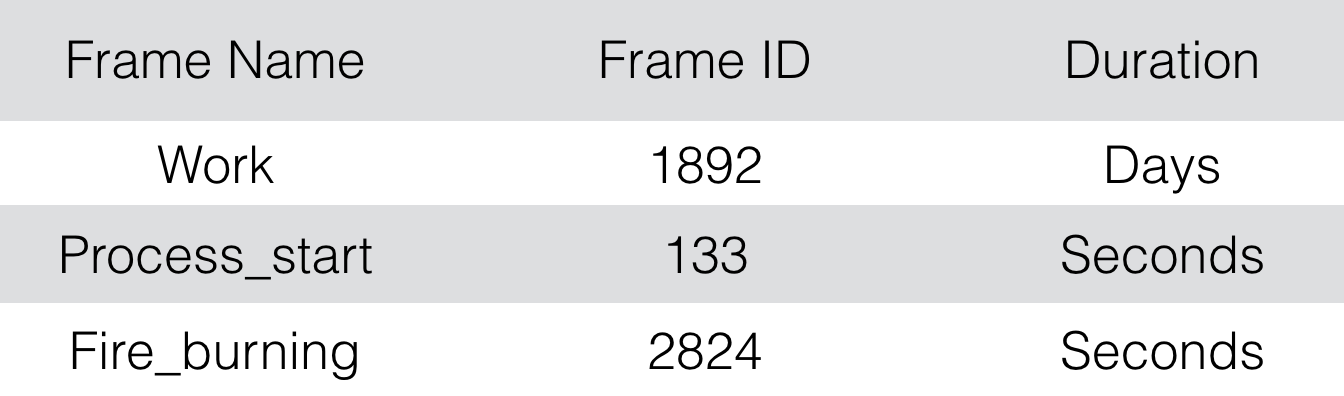
\includegraphics[width=\columnwidth]{figs/fig4.png}}
\caption{Frame duration.}
\label{fourth_fig}
\end{center}
\vskip -0.3in
\end{figure}


\section{The effectiveness of using frame or frame+verb to represent duration}

Before using frame or frame+verb to represent duration, I should first figure out whether frame and frame+verb have any relationship with duration. I will argue that frame and frame+verb both have relationships with duration and frame+verb has stronger relationships.
I mainly consider two parameters to evaluate the effectiveness of using frame or frame+verb to represent duration.

\textbf{1)} The first one is, in average a frame correspond to how many durations. In the best situation, I hope a frame only correspond to one duration, so the frame and the duration have a very strong connection. This value should between 1 and 7, and the smaller the better.

\textbf{2)} The second one is, the weight of the most frequent duration of the frame. This value equals to 

\[Weight =  \frac{\sum_{num} mostFrequentDuration}{\sum_{num} allDuration}\]
This value should between 1/7 and 1, the bigger the better.
There are 132 frames and 192 frame+verb extracted from 553 annotated sentences which explicitly contain duration information.

\begin{figure}[H] 
\begin{center} 
\centerline{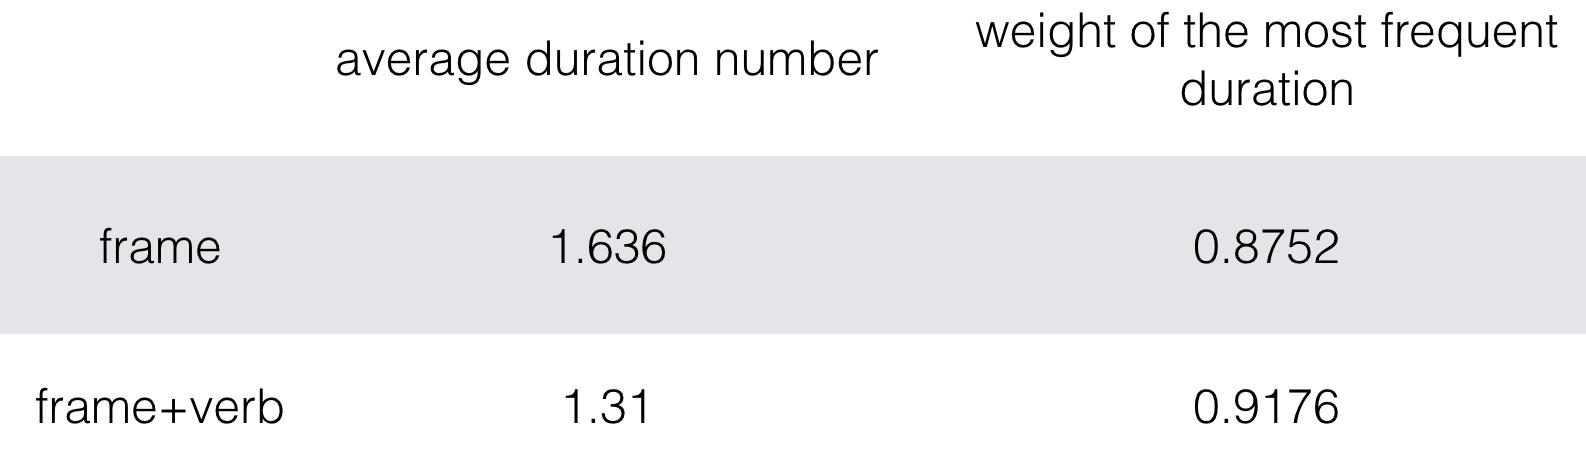
\includegraphics[width=\columnwidth]{figs/fig5.png}}
\caption{Consider all frame and frame+verb, the average duration number and the weight of the most frequent duration.}
\label{fifth_fig}
\end{center}
\vskip -0.3in
\end{figure}

It seems that the two corpus both perform very well in these two parameters. However, we should consider that our dataset is quite small, which means many frames or frame+verbs only appear once. The average duration numbers and the weight of the most frequent durations of these frames or frame+verbs which only appear once are 1. The two parameters are both quite perfect, however, it is not because frames or frame+verbs perform well on these samples, but these samples only appear once. So the two parameters are naturally to be 1. 
So next, I only consider the frames or frame+verbs which appear more than one time.

\begin{figure}[H] 
\begin{center} 
\centerline{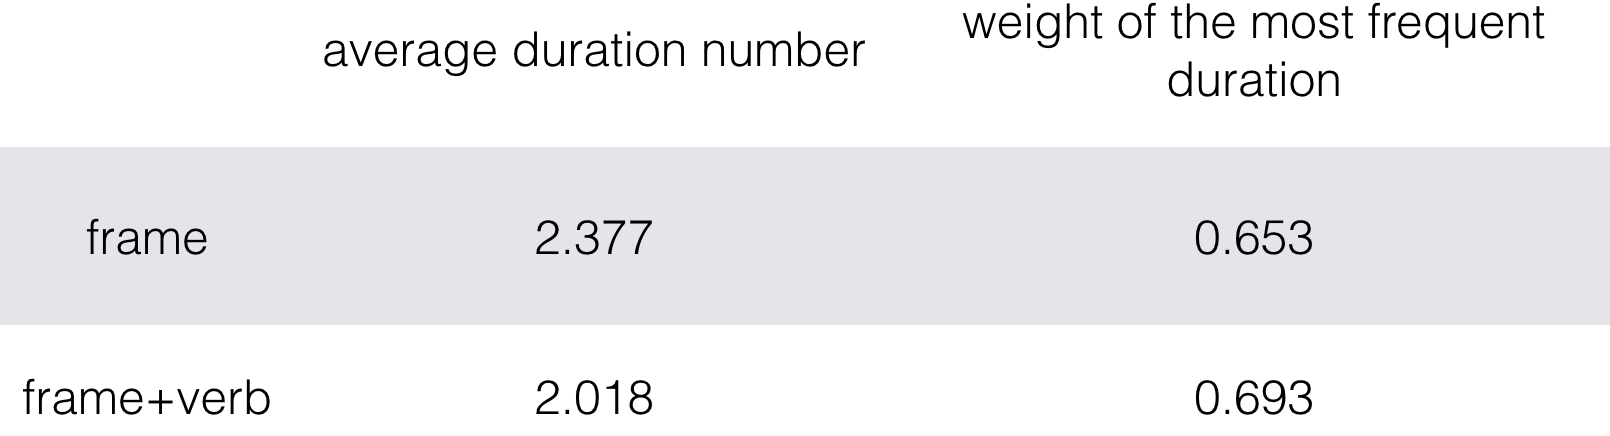
\includegraphics[width=\columnwidth]{figs/fig6.png}}
\caption{\textbf{Only consider the frames and frame+verbs that appear more than one time.} The average duration number and the weight of the most frequent duration.}
\label{sixth_fig}
\end{center}
\vskip -0.3in
\end{figure}

I think under this situation, the two parameters are closer to reality. We can see that although frame and frame+verb both perform worse on these two parameters, they still perform much better than baseline. So we can say that frame and frame-verbs both have relationships with durations.
In addition, I want to also evaluate another two parameters.
How many frames or frame+verbs that appear more than one time correspond to only one duration.
The number of the frames or frame+verbs that appear more than one time. 


\begin{figure}[H] 
\begin{center} 
\centerline{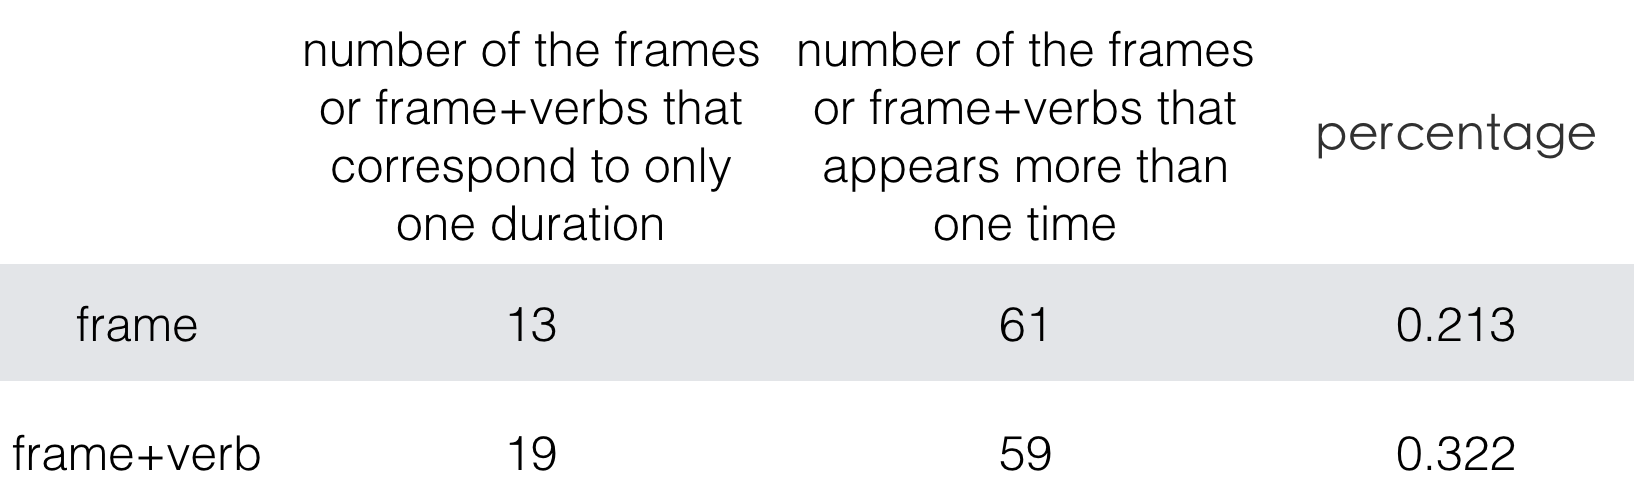
\includegraphics[width=\columnwidth]{figs/fig7.png}}
\caption{Among these samples that appear more than one time, how many of them correspond to only one duration.}
\label{seventh_fig}
\end{center}
\vskip -0.3in
\end{figure}


\section{Confusion matrix and result analyses}

The testing dataset has 50 sample extracted from 110 annotated sentences. My strategy of doing partial match is:

\textbf{1)} If frame matches and LU does not match. I will use the frame to predict duration.

\textbf{2)} If LU matches and frame does not match. I will search if the frame's parent or child frame
matches. I will consider the parent frame and child frame shares the same duration. If the frame's parent frame or child frame also not match, I will consider I can't predict its duration and abandon it.

The size of training data is 167 frame-verbs and 120 frames. Base on these training data I should predict 50 samples' duration, but I can only predict 34 samples' duration. And the confusion matrix shows as below:


\begin{figure}[H] 
\begin{center} 
\centerline{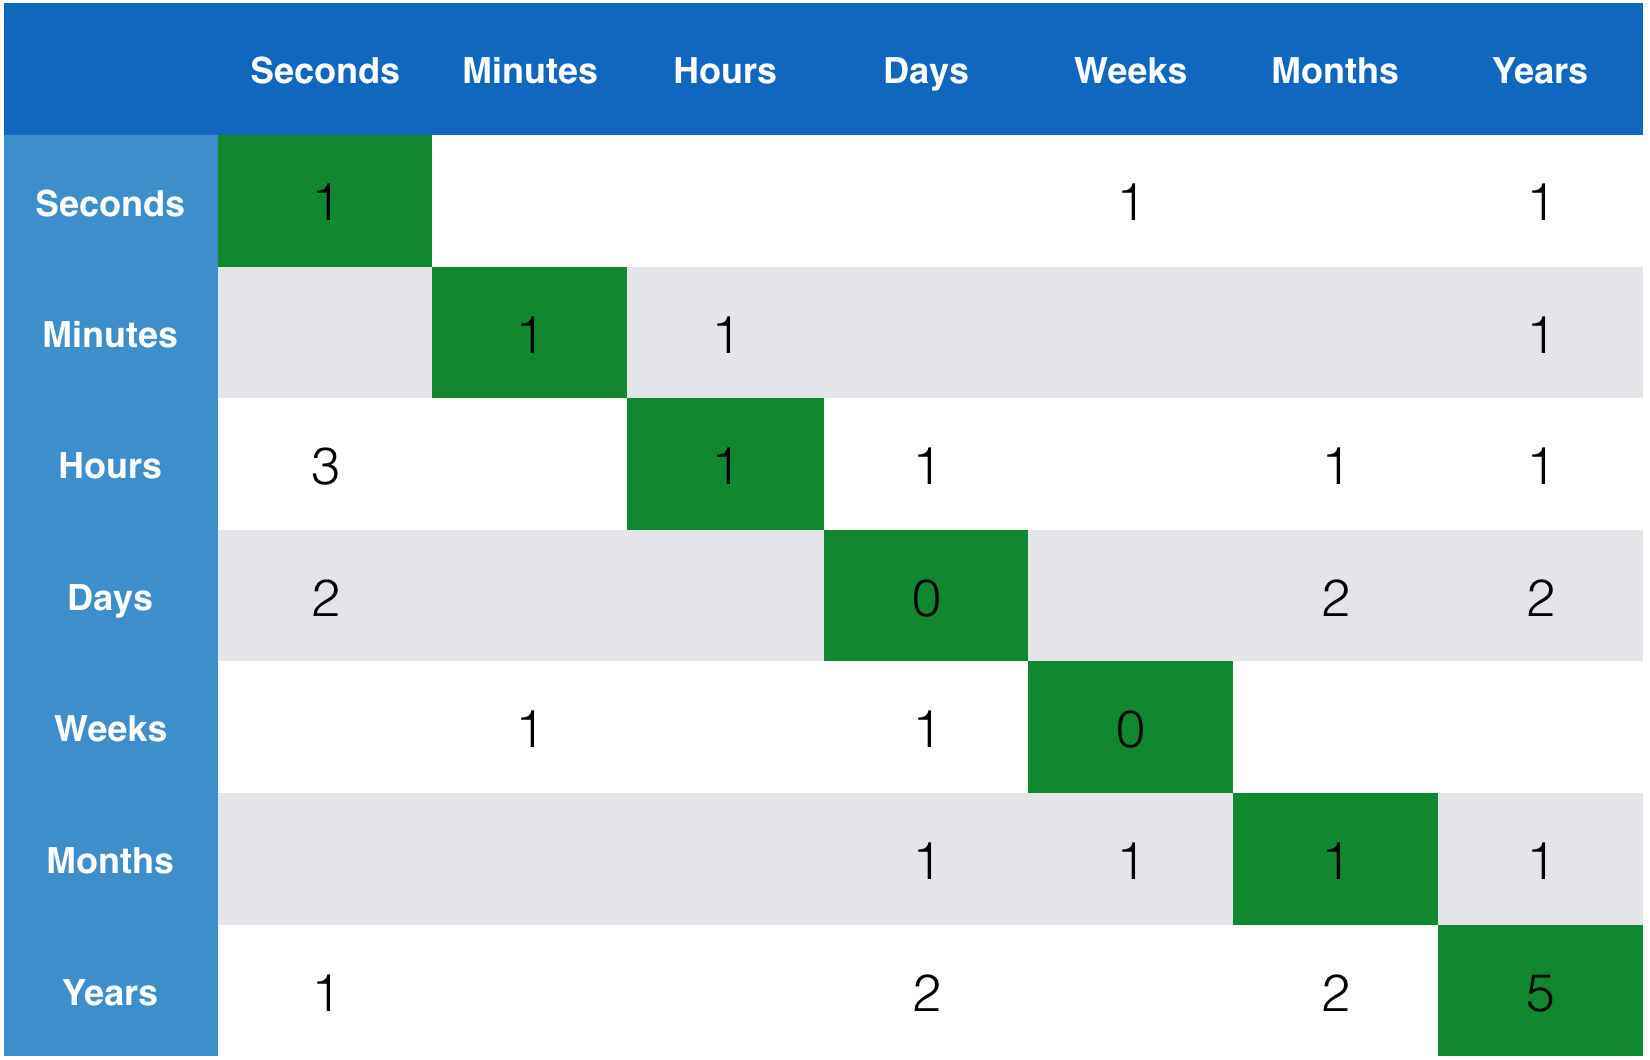
\includegraphics[width=\columnwidth]{figs/fig8.png}}
\caption{Confusion matrix.}
\label{eighth_fig}
\end{center}
\vskip -0.3in
\end{figure}


11 samples are predicted larger than the correct value and 14 samples are predicted smaller than the correct value. The prediction accuracy is 9/34 = 0.265. The prediction accuracy is low and there is no obvious trend that the predictions are always bigger or smaller than correct values. But we can notice that there are 6 predictions are close to correct value. 
I think the lack of training data and the not strong connection between frame, frame-verb, and duration both lead to this poor performance. I think next I should collect more data to enrich our frame and frame-verb duration corpus and I should consider frame elements when I do duration prediction. So maybe next I should build a frame-verb-element duration corpus.

\end{document}
